% Establish the teritory, the importance and reviewing previous work. how does this assignment relate to cyber-security
\section{Introduction}

Recently in the Harvard Business Review (HBR) \textcite{Milica:2023} identified the challenges regarding cyber-security oversight by boards.  The
authors went on propose a strategic enhancement for Chief Information Security Officers (CISOs).

The life of a cyber-security professional can be a thankless task at times. Even with cyber-security spend increasing as a percentage of IT
budgets \autocite{Hiscox:2022}, boards are reporting that they are not seeing eye-to-eye with their CISOs where \enquote{65\% of board members
  think their organization is at risk of a material cyberattack, only 48\% of CISOs share that view.} and that
this \enquote{communication gap and board-CISO misalignment hinders progress in cybersecurity} 

In light of the challenges identified in the Harvard Business Review article regarding cybersecurity oversight by boards, this report seeks to address these issues and propose a strategic enhancement for Chief Information Security Officers (CISOs). The key concerns include:

\subsection{CISO Challenges in Cybersecurity Oversight by Boards}

\begin{enumerate}
\item Disconnect Between Boards and CISOs:
     \begin{itemize}
        \item Limited alignment between boards and CISOs.
        \item Insufficient interaction hindering meaningful cybersecurity discussions.
        \item Communication gaps and misalignment impeding progress in cybersecurity.
     \end{itemize}
 
\item Focus on Protection Over Resilience:
     \begin{itemize}
        \item Boards prioritizing cyber protection despite a high perceived risk.
        \item Investments in protection not directed to critical areas.
        \item Advocacy for a shift towards organizational resilience.
     \end{itemize}
 
\item Cybersecurity as a Technical Topic:
     \begin{itemize}
        \item Boards viewing cybersecurity primarily as a technical issue.
        \item Limited time in board meetings making it challenging to address nuances.
        \item Need for a shift from technical to management challenges in discussions.
     \end{itemize}
 
\item Board Composition and Expertise:
     \begin{itemize}
        \item Many boards lacking cybersecurity expertise.
        \item SEC proposing explicit cybersecurity recommendations for boards.
        \item Necessity for board composition changes to incorporate cybersecurity knowledge.
     \end{itemize}
 
\item Priority and Commitment:
     \begin{itemize}
        \item A quarter of boardrooms not viewing cybersecurity as a priority.
        \item Inadequate frequency of cybersecurity discussions.
        \item The necessity of making cybersecurity a continuous priority with ongoing commitment.
     \end{itemize}
\end{enumerate}

Organisations are clearly spending more on cyber-security.  Financial damage is going up. But the HBR report highlights a focus on prevention rather than resiliency.  
   
\begin{figure}[!ht] % Single column figure
  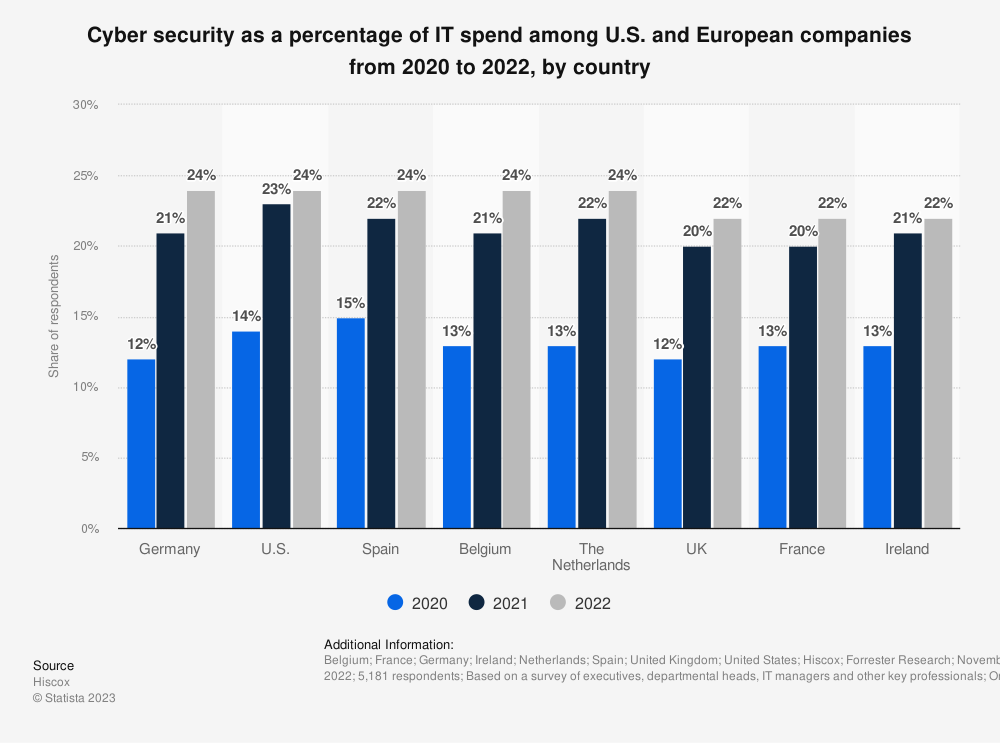
\includegraphics[width=0.95\textwidth]{statistic_id1245356_share-of-it-spend-on-cyber-security-in-the-us-and-europe-2020-2022-by-country.png}\hfill
  \caption{Spending on Cyber Security  \autocite{Hiscox:2022}  Source: Statistica Inc.}
  \label{fig:cybersecurity-spending}
\end{figure}

\begin{figure}[!ht] % Single column figure
  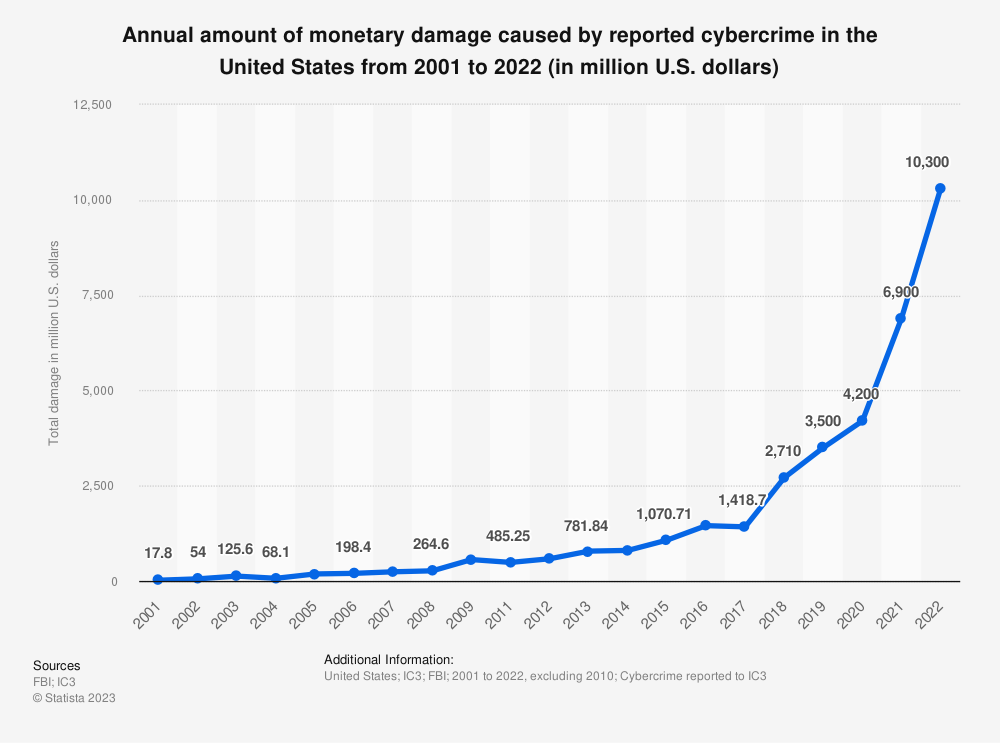
\includegraphics[width=0.95\textwidth]{statistic_id267132_annual-amount-of-financial-damage-caused-by-reported-cybercrime-in-us-2001-2022.png}\hfill
  \caption{Financial Damage caused by Cybercrime in the USA year-on-year \autocite{FBI:2023} Source: Statistica Inc.}
  \label{fig:cybercrime-cost}
\end{figure}


   
\subsection{The CISO and current state of malware attacks on Windows.}

\textbf{Importance of addressing issues in cybersecurity oversight by boards}.

To address these challenges, this report proposes a strategic proposition aimed at enhancing the CISO's position within the organization. The proposition includes:


\begin{enumerate}
      \item Engagement with Senior Executives:
         \begin{itemize}
            \item Demonstrating the importance of cybersecurity as an organizational imperative.
            \item Building personal relationships with senior executives to bridge the communication gap.
         \end{itemize}
         
      \item Explanation of Cyber-Resilience Program:
         \begin{itemize}
            \item Clearly communicating the organization's cyber-resilience strategy.
            \item Translating technical jargon into business language for better understanding by the board.
         \end{itemize}
         
      \item Initiatives within the Department:
         \begin{itemize}
            \item Developing regular cybersecurity reports to provide transparent insights.
            \item Showcasing the department's efforts in enhancing cyber resilience.
         \end{itemize}
         
      \item Use Case Report on Process Injection Attacks:
         \begin{itemize}
            \item Presenting a real-world use case demonstrating new process injection attacks.
            \item Evaluating the effectiveness of the organization's Endpoint Detection Response system (EDR).
         \end{itemize}
         
      \item Ensuring EDR Vendor Adaptation:
         \begin{itemize}
            \item Using the use case report to ensure the EDR vendor is adapting to new threats.
            \item Strengthening the organization's defense mechanisms against evolving cyber threats.
         \end{itemize}
\end{enumerate}


This comprehensive approach aims not only to address the challenges outlined in the Harvard Business Review article but also to elevate the CISO's role by fostering better understanding, engagement, and preparedness within the organization. cite \href{https://www.cisa.gov/cross-sector-cybersecurity-performance-goals}{cross-sector-cybersecurity-performance-goals} and 


% Identify a niche, indicating a gap in in knowledge

Relying on EDR systems as a principle defence against a myriad of attacks alieviates many problems.  But it does not alievate the communication gap between company boards
and the cyber and information security professionals that protect their organisation.  CISOs need to understand the threat landscape, their mitigants to attacks, and
where failures in their own security systems may fail.  Having new internal analysis and being fully abreast of the threats, vulnerabilities and mitigants of their
systems will equip our CISO with the information they need to formulate and communicate a set of action/response readiness to the senior executives and board members. 

\subsection{Introducing Mockingjay: Importance of understanding process injection techniques.}

This cat-and-mouse game beween security groups on the one hand, and the evasion and increased sophistication and novelty on the part of malicious actors on the other \ldots
\textit{introduce EDR} \ldots
For vendors of EDR, MDR \& XDR solutions investigating existing and emerging threats is an on-going process \href{https://research.tue.nl/files/305661196/Olteanu_I.C..pdf}{evaluating the response effectiveness of their XDR technology}.


% Occupy the niche; purpose of new research, listing questions, the value of the work and the structure of the writing
\subsection{Purpose of the report: proposing a strategic enhancement for CISOs.}

This paper is a model for the types of analysis that a CISO should be requesting from their information security teams.  This paper reports on a new process injection technique \autocite{Peixoto:2023} in relation to the protections offered by EDR and XDR technologies, and specifically with behaviours that could be used to detect API attacks \autocite{Wang:2022}.

We will analyse the ``Mockingjay'' attack and identify the defences offered by modern XDR systems and ask if there's a credible chance of evading detection.  By looking at an implementation of the attack we will ask in what ways a threat detection system strengthen it's defences, and what artifacts could be automatically produced that could demonstrate any anomoly in a systems behaviour. 

Section 2 to put our case study on the Mockingjay in context, we review the background of the process injection technique and how it was weaponised by malware authors.

Section 3 we then look at the changing landscape of threat actors and defense mitigants to understand how this is a contantly evolving landscape.  Endpoint Defence Response (EDR) security that is typically relied upon to prevent these types of attack.  We will then look at methods a identifying these attacks and look at the likelihood of Endpoint Security products of identifying the attack.   An investigation into the Mockingjay attack and against a recently published paper ``Procguard'' \autocite{Wang:2022} and asks whether this attack method would lickly be caught.

Section 5 is a case study on the Mockingjay process injection attack that a CISO should be expecting from their team.  It will crystalise challenges
that our titular CISO should be engaging his vendor on.  It should also feed back into the cyber-security playbooks that the organisation has, and
the threat and response reported back to senior executives and boards.

%to use reinforcement to identify ``RWX'' code injections that should be part of a corporations EDR solution.
% {jwang,mcj123,ZiangLi,2018302180148,iwangjye}@whu.edu.cn

Section 5 is an implementation of the attack and will look at manually identifying an infected process and generating artifacts that could be used in automating the process.

Section 6 is an evaluation section, reflecting on the project.

Section 7 is the conclusion and will suggest risks and mitigants for process injection attacks and further research that could be undertaken to adapt to
and mitigate evolving cyber-security threats.